\chap{Introduction}
% Fancy a quote?
\begin{flushright}
  \textit{Everything should be made as simple as possible, but not simpler.}\\
  {---Albert Einstein}
\end{flushright}

\section{Background}

With modern advances in science and technology, statistical models and the data on which they are fit are becoming increasingly complex. Data sets are expanding in size, often both in terms of the number of variables (features) as well as the number of observations. In some fields, this growth in complexity has been paralleled with more effective methods with which to collect observations, as in, for instance, crowd science and social media data. But in other areas, collecting data still amounts to a costly endeavor. In bioinformatics, for example, ethical concerns and rising requirements on the quality of data have only served to \emph{raise} the costs of data collection. And as a result, the data collected in these fields is becoming \emph{wider}: the ratio between the number of variables (features) and the number of observations is increasing~(\Cref{tab:types-of-data}).

\begin{table}[htbp]
  \caption{Tall and wide data. Each row is an observation, for instance the measurement on a person in a study, and each column (feature) represents all the measurements on a variable for all the observations.}
  \label{tab:types-of-data}
  \begin{subtable}{.5\linewidth}\centering
    \caption{Tall data}\label{tab:1b}
    {\begin{tabular}{ccc}
        \toprule
        $\vec{x}_1$ & $\vec{x}_2$ & $\vec{x}_3$ \\
        \midrule
        0           & 0.32        & 1           \\
        1           & 1           & -1          \\
        $\vdots$    & $\vdots$    & $\vdots$    \\
        \bottomrule
      \end{tabular}}
  \end{subtable}
  \begin{subtable}{.5\linewidth}\centering
    \caption{Wide data}
    {\begin{tabular}{cccc}
        \toprule
        $\vec{x}_1$ & $\vec{x}_2$ & $\vec{x}_3$ & $\cdots$ \\
        \midrule
        0           & 0.32        & 1           & $\cdots$ \\
        1           & 1           & -1          & $\cdots$ \\
        \bottomrule
      \end{tabular}}
  \end{subtable}%
\end{table}

The growth in the number of observations is a luxury problem, since it, at least as far as the model is concerned, provides only benefit\footnote{The downsides are generally only related to computational issues, such as storing and processing this data.}. But an expansion in the number of features (wider data) is a more delicate issue. The problem is that if all the features that we have collected are important, but to varying degree, then we are out of luck as far as understanding our data goes. Instead we have to more or less hope that there is a \emph{sparse} representation~(\Cref{fig:sparse-signal}) of our data that, with some acceptable loss of information, allows us to understand the problem that we are studying.

\begin{figure}[htpb]
  \centering
  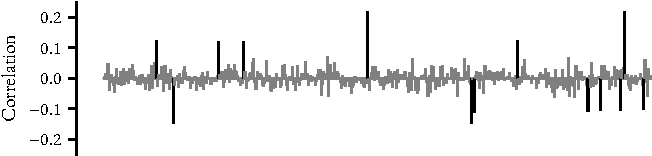
\includegraphics[]{figures/sparse-signal.pdf}
  \caption{%
    A relatively sparse signal. The plot shows standard Pearson correlations between the response vector \(\vec{y}\) and each feature in the \data{madelon} data set~\parencite{guyon2004}. Correlations above 0.1 have been colored in black, the rest in gray.
  }
  \label{fig:sparse-signal}
\end{figure}

We call this hope the \emph{sparsity assumption}. And it can be motivated through the \emph{bet-on-sparsity principle}: assume that the underlying model is sparse and use a sparse method to model it. If the assumption is correct, then our method has a chance of doing well. But if the assumption is incorrect, then our method will not work---but no other method would~\parencite{hastie2009}.

The success of neural networks and other complex models that model high-dimensional data well yet do not enforce sparsity does raise questions as to the validity of this principle. But in our setting, which, loosely speaking, is \emph{explainable} methods for regression, it still bears relevance.

Technically speaking, we are interested in data sets that are made up of a \(n \times p\) matrix of features \(\mat{X}\) and a response vector of length \(n\), \(\vec{y}\):
\[
  \mat{X} = \begin{bmatrix}
    1.5     & 0.3     & \cdots & x_{1,p} \\
    -0.9    & 0.1     & \cdots & x_{2,p} \\
    \vdots  & \vdots  & \ddots & \vdots  \\
    x_{n,1} & x_{n,2} & \cdots & x_{n,p} \\
  \end{bmatrix},\qquad
  \vec{y} = \begin{bmatrix}0.2 \\ -0.9 \\ \vdots \\ y_n\end{bmatrix},
\]
where we have inserted some arbitrary values for the sake of illustration. The data presented in \Cref{tab:types-of-data} corresponds to \(\mat{X}\) here.

In the simplest case, we assume that \(\vec{y}\) is a linear combination of the features in \(\mat{X}\) plus some noise, for instance measurement noise, which we write mathematically as
\[
  \vec{y} = \mat{X}\vec{\beta} + \beta_0 + \vec{\varepsilon},
\]
where \(\vec{\beta}\) is a vector of coefficients and \(\beta_0\) the \emph{intercept}. In this representation of the data, the coefficients \(\vec{\beta}\) are the parameters that we are interested in estimating and represent the effect each feature has on the response vector \(\vec{y}\).

Assuming this model is correct, a natural choice of model to fit this data with is linear regression, which is in fact exactly the model above provided that we, in addition, also assume that the noise \(\vec{\varepsilon}\) is normally distributed\footnote{Tecnically, this not in fact a core assumption of linear regression, but it is necessary for certain aspects of it.} with mean zero and constant variance.

Since in the presence of noise there generally exists no \(\beta\) that will fit the data perfectly, we must accept that the model is only an approximation. The natural follow-up question is then: what \emph{is} a good approximation? To answer this question, we need to define some measure of error. The most common measure, at least as far as linear regression models go, is by far the sum of squared errors between the predicted response vector
\[
  \hat{\vec{y}} = \mat{X}\hat{\vec{\beta}}
\]
and the true response vector \(\vec{y}\), that is
\[
  \lVert \vec{y} - \hat{\vec{y}}\rVert^2_2 = \sum_{i=1}^n (y_i - \hat{y}_i)^2.
\]
The smaller this measure, the better the fit. Which means that we can pose the problem of finding the best model as the following optimization problem:
\[
  \begin{aligned}
     & \text{minimize} &  & \frac{1}{2} \lVert \vec{y} - \mat{X}\vec{\beta}\rVert^2_2.
  \end{aligned}
\]
The factor of \(1/2\) is included for convenience, for reasons that will become clear later on.
This choice leads to the ordinary least-squares (OLS) regression model, which, for a simple case of a single feature, we have illustrated in \Cref{fig:ols}. There are many other ways to measure error, which all lead to different models, but in this thesis we will focus on the method of least squares.

The most common linear regression model is ordinary least-squares regression~(OLS), in which we  then the model that minimizes the sum of the squared residuals between the response vector \(\vec{y}\) and the predictions (\(\hat{\vec{y}}\)) made by the model. For the simple case of a single feature, this model is illustrated in \Cref{fig:ols}.

\begin{figure}
  \centering
  \subcaptionbox{%
    The slope of the orange line is \(\beta\). The point where the line intersects the y-axis is the intercept \(\beta_0\).
  }{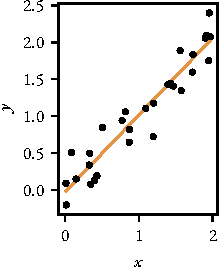
\includegraphics[]{figures/ols-clean.pdf}}\hspace*{1cm}%
  \subcaptionbox{%
    The dotted lines are the residuals and the grey squares are the squared errors.
  }{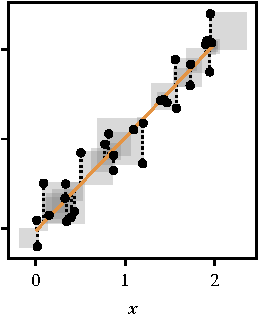
\includegraphics[]{figures/ols-squares.pdf}}
  \caption{%
    Simple ordinary least-squares linear regression for a one-feature problem. }
  \label{fig:ols}
\end{figure}

If have many more observations than features (\(n \gg p\)), then this model might just do. But if we have many more features than observations (\(p \gg n\)), then we have a problem. The problem is that the model will be able to fit the data perfectly, but it will not generalize well to new data. This is because the model will be able to fit the noise in the data, and not the underlying signal. This is called \emph{overfitting}. In fact, the coefficients \(\beta\) will not even be unique in this case.

\begin{figure}
  \centering
  \subcaptionbox{%
    With one fature, the simple ordinarly least-squares regression line fits the data perfectly.
  }{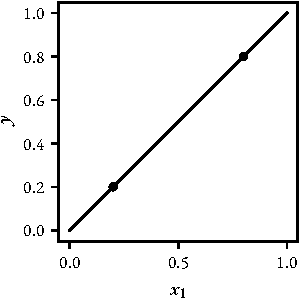
\includegraphics[]{figures/overfit-2d.pdf}}\hfill%
  \subcaptionbox{%
    With two features, multiple fits (planes) will fit the data perfectly.
  }{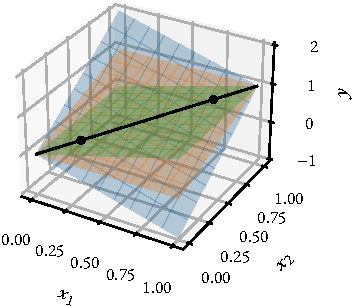
\includegraphics[]{figures/overfit-3d.pdf}}
  \caption{%
    A linear regression problem with two observations
  }
  \label{fig:overfitting}
\end{figure}

The problem illustrated by \Cref{fig:overfitting} is partly one of interpretation. If there are multiple sets of \(\beta\) that will work as well, what do we infer about our parameters?
It is also a case of the curse of dimensionality, in the sense that, as we increase the dimensions of our feature space, our observations start to effectively grow further, and further apart, and occupy less and less of the available space.

In principle, the problem is one of over-parametrization. We have too many parameters for the amount of data that we have. This is, in principle, the same problem that one faces when fitting polynomial regresssion with an increasing number of degress. Eventually the model becomes too flexible and overfits~(\Cref{fig:polyfit}).

\begin{figure}
  \centering
  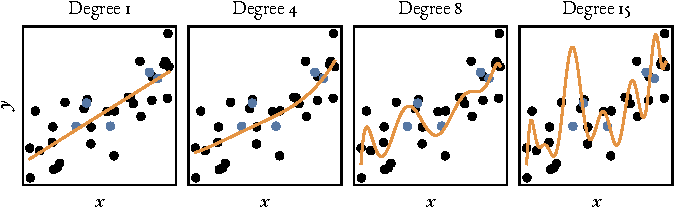
\includegraphics[]{figures/polyfit.pdf}
  \caption{%
    Polynomial regression of a one-feature regression problem.
    The data is generated from the simple linear model \(y_i = 2x_i + \varepsilon\),
    where \(\varepsilon \sim \normal(0, 0.5^2)\).
    The fits to the data become increasingly good as the degree of the polynomial increases, but when new data arrives (the blue points), we see that the model does not generalize well.
  }
  \label{fig:polyfit}
\end{figure}

These problems are the motivation for the use of \emph{regularization} in regression, which we will turn to next.

\section{Regularization}

If the problem is that our model is over-parameterized, which we in the previous section saw is invariably the case when we employ linear regression in the \(p \gg n\) scenario, an intuitive solution might be to restrict or altogheter remove some of the parameters. This is the idea behind \emph{regularization}.

On the surface, this might seem like an awkward idea, since we are in some sense discarding information. But this is exactly what people in the \(n \gg p\) have already done, but at a subjective level. The world is unquestionably high-dimensional and any situation in which we limit the number of features is only an artefact of how we have chosen to measure it. And if we are in the \(n \gg p\) regime, it only means that we have already decided that some features are not important.

Regularization takes another stab at this problem and relies on data, rather than subjective knowledge, in order to choose which features it is that actually matter for the model.

The simplest kind of regularization is called \emph{best-subset selection}, in which we simply set a limit on how many features we allow in our model and fit all possible combinations of models until we find the one that best fits our data. Best subset selection can formally be posed as the following optimzation problem:
% TODO: introduce the minimization objective for OLS somewhere before this
\[
  \begin{aligned}
     & \text{minimize}   &  & \frac{1}{2} \lVert \vec{y} - \mat{X}\vec{\beta}\rVert^2_2, \\
     & \text{subject to} &  & \lVert \vec{\beta} \rVert_0 \leq k,
  \end{aligned}
\]
where \(k\) denotes the number of features that we allow in our model. The \(\lVert \cdot \rVert_0\) norm\footnote{Technically, it's not actually a real norm.} is the number of non-zero elements in a vector.

In other words, if \(k = 2\) and \(p = 3\), for instance, the following models would satisfy our constraints:
\[
  \vec{\beta} = \begin{bmatrix}0 \\ 0 \\ 0\end{bmatrix},\qquad \vec{\beta} = \begin{bmatrix}1 \\ 2 \\ 0\end{bmatrix},\qquad \text{and} \qquad \vec{\beta} = \begin{bmatrix}0 \\ 0 \\ 1\end{bmatrix}.
\]
But the following model would not:
\[
  \vec{\beta} = \begin{bmatrix}1 \\ 2 \\ 3\end{bmatrix}.
\]


There are two problems with this method. The first is that the method involves no shrinkage, which \textcite{stein1956,james1961} in pivotal work asserted was necessary for good performance.

The second is that it is computationally infeasible for large problems. The reason is that the problem is combinatorial and the number of possible models hence grows exponentially with the number of features. Interestingly, \textcite{bertsimas2016} has shown that the problem can actually be written as a mixed-integer optimization problem, which enables the use of modern optimization software. While this is a significant advancement, however, it is still the case that the problem is computationally infeasible for large problems~\parencite{hastie2020}.

% For this thesis, we are in general interested in fitting regularized statistical models to tabular data consisting of a matrix of features (or predictors) \(\mat{X} \in \mathbb{R}^{n \times p}\) and a response vector \(\vec{y} \in \mathbb{R}^n\).
%
% The models that we are interested in fitting are of the form
%
% \begin{align*}
%   \text{minimize} & f(\vec{\beta}; \mat{X}, \vec{y}) = g(\vec{\beta}; \mat{X}, \vec{y}) + h(\vec{\beta})
% \end{align*}
% where \(f(\beta)\)

\subsection{The Lasso}

The perhaps most obvious solution to this problem is to relax the constraint involved in the best-subset selection problem to something that makes the problem easier to solve. And in fact, the closest we can get to the best-subset selection problem without actually solving it is to use the \(\ell_1\) norm in place of the \(\ell_0\) norm. In other words, our problem now becomes
\[
  \begin{aligned}
     & \text{minimize}   &  & \frac{1}{2} \lVert \vec{y} - \mat{X}\vec{\beta}\rVert^2_2, \\
     & \text{subject to} &  & \lVert \vec{\beta} \rVert_1 \leq t,
  \end{aligned}
\]
where \(\lVert \vec{\beta}\rVert_1 = \sum_{j=1}^p |\beta_j|\) and, as a consequence, we have replaced the integer-valued \(k\) with a real-valued (but positive) \(t\). This problem is known as \(\ell_1\)-regularized regression or, more commonly, the \emph{lasso}~\parencite{tibshirani1996}\footnote{The lasso is sometimes written as an acronym (LASSO) for \emph{least absolute shrinkage and selection operator}, but we will stick with the lower-case version here, which the authors themselves use in their recent work.}.

The lasso was introduced to the statistics community by \textcite{tibshirani1996} but actually stems from much earlier research done in the field of signal processing by \textcite{santosa1986}. \textcite{donoho1994,donoho1995} subsequently introduced the concept of the \emph{basis pursuit} problem, which is closely related to the lasso, and developed much of the theoretical framework for the lasso.

We saw previously that the \(\ell_0\) constraint in best-subset selection puts a budget on the number of features allowed in the model. The \(\ell_1\) norm, in contrast, instead puts a budget on the \emph{size} of the coefficients. This leads to both sparsity and shrinkage in the solution. In \Cref{fig:lasso-ball}, we have visualized how this constraint affects the solution of the least-squares objective.

\begin{figure}
  \centering
  \subcaptionbox{A sparse solution, \(\vec{\beta}=[0,-1]^\intercal\).}{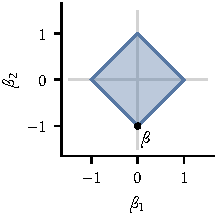
\includegraphics[]{figures/lasso-ball-sparse.pdf}}\hfill%
  \subcaptionbox{A dense solution, \(\vec{\beta}=[0.5,0.5]^\intercal\).}{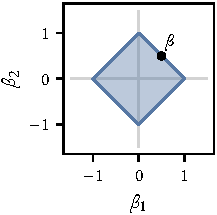
\includegraphics[]{figures/lasso-ball-dense.pdf}}\hfill%
  \subcaptionbox{A solution in which the constraint is inactive, \(\vec{\beta} = [0.4,0.3]^\intercal\). \(t\) is too small to have any effect on the solution.}{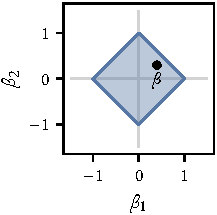
\includegraphics[]{figures/lasso-ball-inactive.pdf}}

  \caption{%
    The \(\ell_1\) norm ball in \(\mathbb{R}^2\) with some possible solutions indicated by \(\vec{\beta}\). The \(\ell_0\) ball (for best-subset selection) and \(k = 1\) would be lines of infinite length. along both of the axes.
  }
  \label{fig:lasso-ball}
\end{figure}

There is now an extensive body of work on the lasso and it has spawned many different variants, such as the fused lasso~\parencite{tibshirani2005}, group lasso~\parencite{yuan2005}, graphical lasso~\parencite{friedman2008}, and square-root lasso~\parencite{belloni2011}. In this thesis, however, we will focus on the standard lasso.

Note, also, that the lasso is also not limited to regularized \emph{linear} regression but can also be used for the entire family of generalized linear models, such as logistic, Poisson, multinomial, and multivariate regression, as well as survival models such as Cox regression. The use of the \(\ell_1\)-norm penalty has also found its way into many other areas of statistics, signal processing, and machine learning, such as matrix factorization, clustering, and deep learning.

% TODO: talk about the lasso path

% TODO: insert figure of lasso path

\subsection{Elastic Net}

\subsection{SLOPE}

\section{Solving the Problems}

\subsection{Optimization}

Originally, \textcite{tibshirani1996} proposed to solve the lasso via an iterative method that used a modification of an algorithm from \textcite{lawson1995}, but it scales badly and is inapplicable when \(p > n\).

\subsection{Screening Rules}

\section{Normalization}

\section{Summary of the Papers}

\subsection{Paper \I}

In this paper, we address the challenge of extracting relevant features from data sets where the number of observations, n, is significantly smaller than the number of predictors, p. We focus on the Sorted L-One Penalized Estimation (SLOPE)—a generalization of the lasso—as a promising method in this context. However, current numerical procedures for SLOPE lack the efficiency that lasso tools possess, especially when estimating a complete regularization path. A key component of lasso's efficiency is predictor screening rules, which allow predictors to be discarded before model estimation. This paper is the first to establish such a rule for SLOPE. We develop a SLOPE screening rule by examining its subdifferential and demonstrate that this rule is a generalization of the strong rule for the lasso. Although our rule is heuristic and may occasionally discard predictors erroneously, we show that such instances are rare and can be easily safeguarded against by a simple check of the optimality conditions. Our numerical experiments reveal that the rule performs well in practice, leading to significant improvements for data in the \(p \gg n\) domain, and incurs no additional computational overhead when \(n > p\). This paper, therefore, presents a significant advancement in the efficiency of SLOPE, particularly in high-dimensional settings.

\subsection{Paper \II}

In this paper, we focus on the lasso, a widely used method for inducing shrinkage and sparsity in the solution vector of regression problems, especially when the number of predictors outweighs the number of observations. Solving the lasso in such high-dimensional settings can be computationally challenging. However, this challenge can be mitigated through the use of screening rules that discard predictors before fitting the model, resulting in a reduced problem. We introduce a new screening strategy, termed look-ahead screening. This method employs safe screening rules to identify a range of penalty values for which a specific predictor cannot enter the model, thereby screening predictors along the remaining path. Our experiments demonstrate that these look-ahead screening rules outperform the active warm-start version of the Gap Safe rules, marking a significant advancement in the efficiency of solving high-dimensional lasso problems.

\subsection{Paper \III}

In this paper, we address the challenge of predictor screening rules in l1-regularized regression problems, such as the lasso. These rules, which eliminate predictors from the design matrix before fitting a model, have significantly improved the speed of solving such problems. However, current state-of-the-art screening rules struggle with highly-correlated predictors, often becoming overly conservative. To tackle this issue, we introduce a new screening rule: the Hessian Screening Rule. This rule leverages second-order information from the model to provide more accurate screening and higher-quality warm starts. Our proposed rule outperforms all other alternatives we studied on datasets with high correlation for both l1-regularized least-squares (the lasso) and logistic regression. It also delivers the best performance overall on the real datasets we examined. This paper, therefore, presents a significant advancement in dealing with highly-correlated predictors in l1-regularized regression problems.

\subsection{Paper \IV}

In this paper, we tackle the challenges posed by the rapid development of machine learning research, particularly in the area of numerical validation. Researchers often face a multitude of methods to compare, lack of transparency and consensus on best practices, and the tedious task of re-implementing work. This often results in partial validation, which can lead to incorrect conclusions and hinder research progress. To address these issues, we introduce Benchopt, a collaborative framework designed to automate, reproduce, and publish optimization benchmarks in machine learning across different programming languages and hardware architectures. Benchopt simplifies the benchmarking process by providing a ready-to-use tool for running, sharing, and extending experiments. We demonstrate its wide applicability through benchmarks on three standard learning tasks: $\ell_2$-regularized logistic regression, Lasso, and ResNet18 training for image classification. These benchmarks reveal key practical findings that provide a more nuanced view of the state-of-the-art for these problems, emphasizing that the details matter in practical evaluation. We believe that Benchopt will encourage collaborative work in the community and improve the reproducibility of research findings.

\subsection{Paper \V}

In this paper we delve into the Sorted L-One Penalized Estimation (SLOPE), an extension of the renowned lasso regression method. Despite the promising statistical properties of SLOPE, its adoption has been limited due to the inefficiency of existing algorithms in high-dimensional contexts. To overcome this challenge, we introduce a novel, faster algorithm that solves the SLOPE optimization problem.

Our algorithm merges the techniques of proximal gradient descent and proximal coordinate descent, significantly enhancing the efficiency of the SLOPE method. We also shed new light on the directional derivative of the SLOPE penalty and its associated SLOPE thresholding operator, and provide assurances of convergence for our proposed solver. Through comprehensive benchmarks on both simulated and real data, we demonstrate that our method outperforms a host of competing algorithms. This paper is a significant contribution as it broadens the applicability of the SLOPE method in high-dimensional settings, potentially paving the way for its wider use in the field.

\subsection{Paper \VI}

In this paper, we explore the sensitivity of regularized methods, such as the lasso and ridge regression, to the scales of the features in the data. It's standard practice to normalize features to ensure they share the same scale. While standardization is common for continuous data, binary data, particularly when high-dimensional and sparse, is often not scaled at all. We demonstrate that this choice can significantly impact the estimated model when the binary features are imbalanced, and that these effects also depend on the type of regularization used. Specifically, we show that the size of a feature's corresponding coefficient in the lasso is directly related to its class imbalance, and this effect depends on the normalization used. We propose potential solutions to this issue and discuss the case when data is mixed, containing both continuous and binary features. This paper, therefore, provides valuable insights into the impact of feature scaling on regularized methods and offers practical solutions for handling mixed data.
